% Options for packages loaded elsewhere
\PassOptionsToPackage{unicode}{hyperref}
\PassOptionsToPackage{hyphens}{url}
%
\documentclass[
]{article}
\usepackage{amsmath,amssymb}
\usepackage{lmodern}
\usepackage{iftex}
\ifPDFTeX
  \usepackage[T1]{fontenc}
  \usepackage[utf8]{inputenc}
  \usepackage{textcomp} % provide euro and other symbols
\else % if luatex or xetex
  \usepackage{unicode-math}
  \defaultfontfeatures{Scale=MatchLowercase}
  \defaultfontfeatures[\rmfamily]{Ligatures=TeX,Scale=1}
\fi
% Use upquote if available, for straight quotes in verbatim environments
\IfFileExists{upquote.sty}{\usepackage{upquote}}{}
\IfFileExists{microtype.sty}{% use microtype if available
  \usepackage[]{microtype}
  \UseMicrotypeSet[protrusion]{basicmath} % disable protrusion for tt fonts
}{}
\makeatletter
\@ifundefined{KOMAClassName}{% if non-KOMA class
  \IfFileExists{parskip.sty}{%
    \usepackage{parskip}
  }{% else
    \setlength{\parindent}{0pt}
    \setlength{\parskip}{6pt plus 2pt minus 1pt}}
}{% if KOMA class
  \KOMAoptions{parskip=half}}
\makeatother
\usepackage{xcolor}
\usepackage[margin=1in]{geometry}
\usepackage{color}
\usepackage{fancyvrb}
\newcommand{\VerbBar}{|}
\newcommand{\VERB}{\Verb[commandchars=\\\{\}]}
\DefineVerbatimEnvironment{Highlighting}{Verbatim}{commandchars=\\\{\}}
% Add ',fontsize=\small' for more characters per line
\usepackage{framed}
\definecolor{shadecolor}{RGB}{42,33,28}
\newenvironment{Shaded}{\begin{snugshade}}{\end{snugshade}}
\newcommand{\AlertTok}[1]{\textcolor[rgb]{1.00,1.00,0.00}{#1}}
\newcommand{\AnnotationTok}[1]{\textcolor[rgb]{0.00,0.40,1.00}{\textbf{\textit{#1}}}}
\newcommand{\AttributeTok}[1]{\textcolor[rgb]{0.74,0.68,0.62}{#1}}
\newcommand{\BaseNTok}[1]{\textcolor[rgb]{0.27,0.67,0.26}{#1}}
\newcommand{\BuiltInTok}[1]{\textcolor[rgb]{0.74,0.68,0.62}{#1}}
\newcommand{\CharTok}[1]{\textcolor[rgb]{0.02,0.61,0.04}{#1}}
\newcommand{\CommentTok}[1]{\textcolor[rgb]{0.00,0.40,1.00}{\textbf{\textit{#1}}}}
\newcommand{\CommentVarTok}[1]{\textcolor[rgb]{0.74,0.68,0.62}{#1}}
\newcommand{\ConstantTok}[1]{\textcolor[rgb]{0.74,0.68,0.62}{#1}}
\newcommand{\ControlFlowTok}[1]{\textcolor[rgb]{0.26,0.66,0.93}{\textbf{#1}}}
\newcommand{\DataTypeTok}[1]{\textcolor[rgb]{0.74,0.68,0.62}{\underline{#1}}}
\newcommand{\DecValTok}[1]{\textcolor[rgb]{0.27,0.67,0.26}{#1}}
\newcommand{\DocumentationTok}[1]{\textcolor[rgb]{0.00,0.40,1.00}{\textit{#1}}}
\newcommand{\ErrorTok}[1]{\textcolor[rgb]{1.00,1.00,0.00}{\textbf{#1}}}
\newcommand{\ExtensionTok}[1]{\textcolor[rgb]{0.74,0.68,0.62}{#1}}
\newcommand{\FloatTok}[1]{\textcolor[rgb]{0.27,0.67,0.26}{#1}}
\newcommand{\FunctionTok}[1]{\textcolor[rgb]{1.00,0.58,0.35}{\textbf{#1}}}
\newcommand{\ImportTok}[1]{\textcolor[rgb]{0.74,0.68,0.62}{#1}}
\newcommand{\InformationTok}[1]{\textcolor[rgb]{0.00,0.40,1.00}{\textbf{\textit{#1}}}}
\newcommand{\KeywordTok}[1]{\textcolor[rgb]{0.26,0.66,0.93}{\textbf{#1}}}
\newcommand{\NormalTok}[1]{\textcolor[rgb]{0.74,0.68,0.62}{#1}}
\newcommand{\OperatorTok}[1]{\textcolor[rgb]{0.74,0.68,0.62}{#1}}
\newcommand{\OtherTok}[1]{\textcolor[rgb]{0.74,0.68,0.62}{#1}}
\newcommand{\PreprocessorTok}[1]{\textcolor[rgb]{0.74,0.68,0.62}{\textbf{#1}}}
\newcommand{\RegionMarkerTok}[1]{\textcolor[rgb]{0.74,0.68,0.62}{#1}}
\newcommand{\SpecialCharTok}[1]{\textcolor[rgb]{0.02,0.61,0.04}{#1}}
\newcommand{\SpecialStringTok}[1]{\textcolor[rgb]{0.02,0.61,0.04}{#1}}
\newcommand{\StringTok}[1]{\textcolor[rgb]{0.02,0.61,0.04}{#1}}
\newcommand{\VariableTok}[1]{\textcolor[rgb]{0.74,0.68,0.62}{#1}}
\newcommand{\VerbatimStringTok}[1]{\textcolor[rgb]{0.02,0.61,0.04}{#1}}
\newcommand{\WarningTok}[1]{\textcolor[rgb]{1.00,1.00,0.00}{\textbf{#1}}}
\usepackage{graphicx}
\makeatletter
\def\maxwidth{\ifdim\Gin@nat@width>\linewidth\linewidth\else\Gin@nat@width\fi}
\def\maxheight{\ifdim\Gin@nat@height>\textheight\textheight\else\Gin@nat@height\fi}
\makeatother
% Scale images if necessary, so that they will not overflow the page
% margins by default, and it is still possible to overwrite the defaults
% using explicit options in \includegraphics[width, height, ...]{}
\setkeys{Gin}{width=\maxwidth,height=\maxheight,keepaspectratio}
% Set default figure placement to htbp
\makeatletter
\def\fps@figure{htbp}
\makeatother
\setlength{\emergencystretch}{3em} % prevent overfull lines
\providecommand{\tightlist}{%
  \setlength{\itemsep}{0pt}\setlength{\parskip}{0pt}}
\setcounter{secnumdepth}{5}
\ifLuaTeX
  \usepackage{selnolig}  % disable illegal ligatures
\fi
\IfFileExists{bookmark.sty}{\usepackage{bookmark}}{\usepackage{hyperref}}
\IfFileExists{xurl.sty}{\usepackage{xurl}}{} % add URL line breaks if available
\urlstyle{same} % disable monospaced font for URLs
\hypersetup{
  pdftitle={Titanic},
  pdfauthor={Sholah},
  hidelinks,
  pdfcreator={LaTeX via pandoc}}

\title{Titanic}
\author{Sholah}
\date{2022-10-15}

\begin{document}
\maketitle

{
\setcounter{tocdepth}{2}
\tableofcontents
}
\begin{Shaded}
\begin{Highlighting}[]
\FunctionTok{library}\NormalTok{(tidyverse)}
\end{Highlighting}
\end{Shaded}

\begin{verbatim}
## -- Attaching packages --------------------------------------- tidyverse 1.3.2 --
## v ggplot2 3.3.6      v purrr   0.3.5 
## v tibble  3.1.8      v dplyr   1.0.10
## v tidyr   1.2.1      v stringr 1.4.1 
## v readr   2.1.3      v forcats 0.5.2 
## -- Conflicts ------------------------------------------ tidyverse_conflicts() --
## x dplyr::filter() masks stats::filter()
## x dplyr::lag()    masks stats::lag()
\end{verbatim}

\begin{Shaded}
\begin{Highlighting}[]
\FunctionTok{library}\NormalTok{(ggplot2)}
\FunctionTok{library}\NormalTok{(ggpie)}
\end{Highlighting}
\end{Shaded}

\begin{Shaded}
\begin{Highlighting}[]
\NormalTok{knitr}\SpecialCharTok{::}\FunctionTok{include\_graphics}\NormalTok{(}\StringTok{"titanicsink.jpg"}\NormalTok{)}
\end{Highlighting}
\end{Shaded}

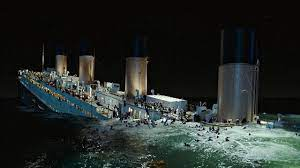
\includegraphics{titanicsink.jpg}

\hypertarget{introduction}{%
\section{INTRODUCTION}\label{introduction}}

here we will explore the data about the passengers of a renowed boat,
RMS Titanic. At the end of this project, we might unfold some facts
about its passengers through this document. For the start, let's import
the data!

\hypertarget{preparing-the-data}{%
\section{PREPARING THE DATA}\label{preparing-the-data}}

\begin{Shaded}
\begin{Highlighting}[]
\NormalTok{tnc }\OtherTok{\textless{}{-}} \FunctionTok{read.csv}\NormalTok{(}\StringTok{"Titanic.csv"}\NormalTok{)}
\end{Highlighting}
\end{Shaded}

\begin{Shaded}
\begin{Highlighting}[]
\FunctionTok{dim}\NormalTok{(tnc)}
\end{Highlighting}
\end{Shaded}

\begin{verbatim}
## [1] 418  12
\end{verbatim}

\begin{Shaded}
\begin{Highlighting}[]
\FunctionTok{head}\NormalTok{(tnc)}
\end{Highlighting}
\end{Shaded}

\begin{verbatim}
##   PassengerId Survived Pclass                                         Name
## 1         892        0      3                             Kelly, Mr. James
## 2         893        1      3             Wilkes, Mrs. James (Ellen Needs)
## 3         894        0      2                    Myles, Mr. Thomas Francis
## 4         895        0      3                             Wirz, Mr. Albert
## 5         896        1      3 Hirvonen, Mrs. Alexander (Helga E Lindqvist)
## 6         897        0      3                   Svensson, Mr. Johan Cervin
##      Sex  Age SibSp Parch  Ticket    Fare Cabin Embarked
## 1   male 34.5     0     0  330911  7.8292              Q
## 2 female 47.0     1     0  363272  7.0000              S
## 3   male 62.0     0     0  240276  9.6875              Q
## 4   male 27.0     0     0  315154  8.6625              S
## 5 female 22.0     1     1 3101298 12.2875              S
## 6   male 14.0     0     0    7538  9.2250              S
\end{verbatim}

\begin{Shaded}
\begin{Highlighting}[]
\FunctionTok{tail}\NormalTok{(tnc)}
\end{Highlighting}
\end{Shaded}

\begin{verbatim}
##     PassengerId Survived Pclass                           Name    Sex  Age
## 413        1304        1      3 Henriksson, Miss. Jenny Lovisa female 28.0
## 414        1305        0      3             Spector, Mr. Woolf   male   NA
## 415        1306        1      1   Oliva y Ocana, Dona. Fermina female 39.0
## 416        1307        0      3   Saether, Mr. Simon Sivertsen   male 38.5
## 417        1308        0      3            Ware, Mr. Frederick   male   NA
## 418        1309        0      3       Peter, Master. Michael J   male   NA
##     SibSp Parch             Ticket     Fare Cabin Embarked
## 413     0     0             347086   7.7750              S
## 414     0     0          A.5. 3236   8.0500              S
## 415     0     0           PC 17758 108.9000  C105        C
## 416     0     0 SOTON/O.Q. 3101262   7.2500              S
## 417     0     0             359309   8.0500              S
## 418     1     1               2668  22.3583              C
\end{verbatim}

\hypertarget{scrutinizing-the-data-types}{%
\subsection{Scrutinizing the data
types}\label{scrutinizing-the-data-types}}

\begin{Shaded}
\begin{Highlighting}[]
\FunctionTok{str}\NormalTok{(tnc)}
\end{Highlighting}
\end{Shaded}

\begin{verbatim}
## 'data.frame':    418 obs. of  12 variables:
##  $ PassengerId: int  892 893 894 895 896 897 898 899 900 901 ...
##  $ Survived   : int  0 1 0 0 1 0 1 0 1 0 ...
##  $ Pclass     : int  3 3 2 3 3 3 3 2 3 3 ...
##  $ Name       : chr  "Kelly, Mr. James" "Wilkes, Mrs. James (Ellen Needs)" "Myles, Mr. Thomas Francis" "Wirz, Mr. Albert" ...
##  $ Sex        : chr  "male" "female" "male" "male" ...
##  $ Age        : num  34.5 47 62 27 22 14 30 26 18 21 ...
##  $ SibSp      : int  0 1 0 0 1 0 0 1 0 2 ...
##  $ Parch      : int  0 0 0 0 1 0 0 1 0 0 ...
##  $ Ticket     : chr  "330911" "363272" "240276" "315154" ...
##  $ Fare       : num  7.83 7 9.69 8.66 12.29 ...
##  $ Cabin      : chr  "" "" "" "" ...
##  $ Embarked   : chr  "Q" "S" "Q" "S" ...
\end{verbatim}

\begin{Shaded}
\begin{Highlighting}[]
\FunctionTok{str}\NormalTok{(tnc)}
\end{Highlighting}
\end{Shaded}

\begin{verbatim}
## 'data.frame':    418 obs. of  12 variables:
##  $ PassengerId: int  892 893 894 895 896 897 898 899 900 901 ...
##  $ Survived   : int  0 1 0 0 1 0 1 0 1 0 ...
##  $ Pclass     : int  3 3 2 3 3 3 3 2 3 3 ...
##  $ Name       : chr  "Kelly, Mr. James" "Wilkes, Mrs. James (Ellen Needs)" "Myles, Mr. Thomas Francis" "Wirz, Mr. Albert" ...
##  $ Sex        : chr  "male" "female" "male" "male" ...
##  $ Age        : num  34.5 47 62 27 22 14 30 26 18 21 ...
##  $ SibSp      : int  0 1 0 0 1 0 0 1 0 2 ...
##  $ Parch      : int  0 0 0 0 1 0 0 1 0 0 ...
##  $ Ticket     : chr  "330911" "363272" "240276" "315154" ...
##  $ Fare       : num  7.83 7 9.69 8.66 12.29 ...
##  $ Cabin      : chr  "" "" "" "" ...
##  $ Embarked   : chr  "Q" "S" "Q" "S" ...
\end{verbatim}

\hypertarget{check-if-there-is-any-missing-value}{%
\subsection{Check if there is any missing
value}\label{check-if-there-is-any-missing-value}}

\begin{Shaded}
\begin{Highlighting}[]
\FunctionTok{anyNA}\NormalTok{(tnc)}
\end{Highlighting}
\end{Shaded}

\begin{verbatim}
## [1] TRUE
\end{verbatim}

\begin{Shaded}
\begin{Highlighting}[]
\FunctionTok{colSums}\NormalTok{(}\FunctionTok{is.na}\NormalTok{(tnc))}
\end{Highlighting}
\end{Shaded}

\begin{verbatim}
## PassengerId    Survived      Pclass        Name         Sex         Age 
##           0           0           0           0           0          86 
##       SibSp       Parch      Ticket        Fare       Cabin    Embarked 
##           0           0           0           1           0           0
\end{verbatim}

\hypertarget{putting-out-the-missing-value-off-the-table}{%
\subsection{Putting out the missing value off the
table}\label{putting-out-the-missing-value-off-the-table}}

\begin{Shaded}
\begin{Highlighting}[]
\NormalTok{tnc }\OtherTok{\textless{}{-}} \FunctionTok{na.exclude}\NormalTok{(tnc)}
\FunctionTok{dim}\NormalTok{(tnc)}
\end{Highlighting}
\end{Shaded}

\begin{verbatim}
## [1] 331  12
\end{verbatim}

\hypertarget{summarizing-the-data}{%
\subsection{Summarizing the data}\label{summarizing-the-data}}

\begin{Shaded}
\begin{Highlighting}[]
\FunctionTok{summary}\NormalTok{(tnc)}
\end{Highlighting}
\end{Shaded}

\begin{verbatim}
##   PassengerId        Survived          Pclass          Name          
##  Min.   : 892.0   Min.   :0.0000   Min.   :1.000   Length:331        
##  1st Qu.: 992.5   1st Qu.:0.0000   1st Qu.:1.000   Class :character  
##  Median :1100.0   Median :0.0000   Median :2.000   Mode  :character  
##  Mean   :1100.2   Mean   :0.3837   Mean   :2.142                     
##  3rd Qu.:1210.5   3rd Qu.:1.0000   3rd Qu.:3.000                     
##  Max.   :1307.0   Max.   :1.0000   Max.   :3.000                     
##      Sex                 Age            SibSp            Parch       
##  Length:331         Min.   : 0.17   Min.   :0.0000   Min.   :0.0000  
##  Class :character   1st Qu.:21.00   1st Qu.:0.0000   1st Qu.:0.0000  
##  Mode  :character   Median :27.00   Median :0.0000   Median :0.0000  
##                     Mean   :30.18   Mean   :0.4834   Mean   :0.3988  
##                     3rd Qu.:39.00   3rd Qu.:1.0000   3rd Qu.:1.0000  
##                     Max.   :76.00   Max.   :8.0000   Max.   :6.0000  
##     Ticket               Fare           Cabin             Embarked        
##  Length:331         Min.   :  0.00   Length:331         Length:331        
##  Class :character   1st Qu.:  8.05   Class :character   Class :character  
##  Mode  :character   Median : 16.00   Mode  :character   Mode  :character  
##                     Mean   : 40.98                                        
##                     3rd Qu.: 40.63                                        
##                     Max.   :512.33
\end{verbatim}

\hypertarget{checking-the-unique-of-each-column}{%
\subsection{Checking the unique of each
column}\label{checking-the-unique-of-each-column}}

\begin{Shaded}
\begin{Highlighting}[]
\FunctionTok{sapply}\NormalTok{(tnc, n\_distinct)}
\end{Highlighting}
\end{Shaded}

\begin{verbatim}
## PassengerId    Survived      Pclass        Name         Sex         Age 
##         331           2           3         331           2          78 
##       SibSp       Parch      Ticket        Fare       Cabin    Embarked 
##           7           7         284         148          73           3
\end{verbatim}

\begin{Shaded}
\begin{Highlighting}[]
\FunctionTok{unique}\NormalTok{(tnc}\SpecialCharTok{$}\NormalTok{Survived)}
\end{Highlighting}
\end{Shaded}

\begin{verbatim}
## [1] 0 1
\end{verbatim}

\begin{Shaded}
\begin{Highlighting}[]
\FunctionTok{unique}\NormalTok{(tnc}\SpecialCharTok{$}\NormalTok{Pclass)}
\end{Highlighting}
\end{Shaded}

\begin{verbatim}
## [1] 3 2 1
\end{verbatim}

\begin{Shaded}
\begin{Highlighting}[]
\FunctionTok{unique}\NormalTok{(tnc}\SpecialCharTok{$}\NormalTok{Sex)}
\end{Highlighting}
\end{Shaded}

\begin{verbatim}
## [1] "male"   "female"
\end{verbatim}

\begin{Shaded}
\begin{Highlighting}[]
\FunctionTok{unique}\NormalTok{(tnc}\SpecialCharTok{$}\NormalTok{Embarked)}
\end{Highlighting}
\end{Shaded}

\begin{verbatim}
## [1] "Q" "S" "C"
\end{verbatim}

Here are some facts and explanation about the data

\begin{enumerate}
\def\labelenumi{\arabic{enumi}.}
\item
  PassengerId is unique for each passenger, there won't be any similar
  passenger id
\item
  Survived contains 2 category. 0 = not survived, 1 = survived
\item
  Pclass is passenger class
\item
  Name, Sex, Age are what they are
\item
  SibSp is the total of siblings on board on the RMS Titanic
\item
  Parch is the total of parents/children on board on the RMS Titanic
\item
  Ticket is the distinctive id for each ticket, or ticket number
\item
  Fare is the ticket price. the mean for the ticket price is 40.98
  dollar and the most expensive ticket charges at 512.33 dollar
\item
  Cabin is the number of Cabin the passenger stayed at (if they were in
  Cabin)
\item
  Embarked is the port of Embarkation. C = Cherbourg, Q = Queenstown; S
  = Southampton
\end{enumerate}

Now, I will remove the columns: SibSp, Parch, as it does not tell much
the relation between each variables or observations

\begin{Shaded}
\begin{Highlighting}[]
\NormalTok{tnc }\OtherTok{\textless{}{-}}\NormalTok{ tnc[,}\SpecialCharTok{{-}}\FunctionTok{c}\NormalTok{(}\DecValTok{7}\SpecialCharTok{:}\DecValTok{8}\NormalTok{)]}
\FunctionTok{names}\NormalTok{(tnc)}
\end{Highlighting}
\end{Shaded}

\begin{verbatim}
##  [1] "PassengerId" "Survived"    "Pclass"      "Name"        "Sex"        
##  [6] "Age"         "Ticket"      "Fare"        "Cabin"       "Embarked"
\end{verbatim}

\hypertarget{data-visualization}{%
\section{3. DATA VISUALIZATION}\label{data-visualization}}

\begin{Shaded}
\begin{Highlighting}[]
\FunctionTok{head}\NormalTok{(tnc)}
\end{Highlighting}
\end{Shaded}

\begin{verbatim}
##   PassengerId Survived Pclass                                         Name
## 1         892        0      3                             Kelly, Mr. James
## 2         893        1      3             Wilkes, Mrs. James (Ellen Needs)
## 3         894        0      2                    Myles, Mr. Thomas Francis
## 4         895        0      3                             Wirz, Mr. Albert
## 5         896        1      3 Hirvonen, Mrs. Alexander (Helga E Lindqvist)
## 6         897        0      3                   Svensson, Mr. Johan Cervin
##      Sex  Age  Ticket    Fare Cabin Embarked
## 1   male 34.5  330911  7.8292              Q
## 2 female 47.0  363272  7.0000              S
## 3   male 62.0  240276  9.6875              Q
## 4   male 27.0  315154  8.6625              S
## 5 female 22.0 3101298 12.2875              S
## 6   male 14.0    7538  9.2250              S
\end{verbatim}

\hypertarget{proportion-of-males-and-females-on-board}{%
\subsection{Proportion of Males and Females On
Board}\label{proportion-of-males-and-females-on-board}}

\begin{Shaded}
\begin{Highlighting}[]
\FunctionTok{ggpie3D}\NormalTok{(}\AttributeTok{data =}\NormalTok{ tnc, }\AttributeTok{group\_key =} \StringTok{"Sex"}\NormalTok{, }
        \AttributeTok{count\_type =} \StringTok{"full"}\NormalTok{, }
        \AttributeTok{tilt\_degrees =} \DecValTok{8}\NormalTok{, }
        \AttributeTok{label\_size=}\DecValTok{2}\NormalTok{) }\SpecialCharTok{+} 
  \FunctionTok{ggtitle}\NormalTok{(}\StringTok{"Percentage Between Males and Females On Board"}\NormalTok{) }\SpecialCharTok{+} 
  \FunctionTok{theme}\NormalTok{(}\AttributeTok{plot.title =} \FunctionTok{element\_text}\NormalTok{(}\AttributeTok{hjust =} \FloatTok{0.5}\NormalTok{))}
\end{Highlighting}
\end{Shaded}

\includegraphics{Titanic_files/figure-latex/unnamed-chunk-17-1.pdf} The
total of males and females recorded in the data, there are 62\% of male
with the total of 204 passengers, and 38\% females with the total of 127
passengers

\hypertarget{ticket-per-class}{%
\subsection{Ticket per Class}\label{ticket-per-class}}

\begin{Shaded}
\begin{Highlighting}[]
\FunctionTok{ggplot}\NormalTok{(tnc, }\FunctionTok{aes}\NormalTok{(Pclass, Fare))}\SpecialCharTok{+}
  \FunctionTok{geom\_col}\NormalTok{(}\FunctionTok{aes}\NormalTok{(}\AttributeTok{fill=}\NormalTok{ Sex), }\AttributeTok{position =} \StringTok{"dodge"}\NormalTok{)}\SpecialCharTok{+}
  \FunctionTok{geom\_jitter}\NormalTok{(}\FunctionTok{aes}\NormalTok{(}\AttributeTok{col=}\NormalTok{Survived, }\AttributeTok{size=}\NormalTok{Fare))}\SpecialCharTok{+}
  \FunctionTok{labs}\NormalTok{(}\AttributeTok{title =} \StringTok{"Ticket Fare per Class of Titanic Passenger"}\NormalTok{, }
       \AttributeTok{x =} \StringTok{"Passenger Class"}\NormalTok{)}\SpecialCharTok{+}
  \FunctionTok{theme}\NormalTok{(}\AttributeTok{plot.title =} \FunctionTok{element\_text}\NormalTok{(}\AttributeTok{hjust =} \FloatTok{0.5}\NormalTok{))}
\end{Highlighting}
\end{Shaded}

\includegraphics{Titanic_files/figure-latex/unnamed-chunk-18-1.pdf} from
the graph above we can see that:

\begin{enumerate}
\def\labelenumi{\arabic{enumi}.}
\item
  the most expensive ticket fare was first class ticket, which was
  bought by female for a total of 500+ dollar
\item
  the cheapest ticket fare was third class ticket, which was bought by
  female for slightly below 50 dollar in total
\item
  there is a passenger of first class without paying a single penny
\item
  the majority of the data is the third class passengers
\item
  there are first class ticket which has the same Fare with second and
  third class, which is under 100 dollars
\item
  the Fare for second and third class are under 100 dollars
\end{enumerate}

Based on insight number \#3, let's uncover who was not paying a single
penny to get on board the RMS Titanic

\begin{Shaded}
\begin{Highlighting}[]
\FunctionTok{filter}\NormalTok{(tnc, Pclass }\SpecialCharTok{==} \DecValTok{1}\NormalTok{, Fare }\SpecialCharTok{==} \DecValTok{0}\NormalTok{)}
\end{Highlighting}
\end{Shaded}

\begin{verbatim}
##   PassengerId Survived Pclass                    Name  Sex Age Ticket Fare
## 1        1264        0      1 Ismay, Mr. Joseph Bruce male  49 112058    0
##         Cabin Embarked
## 1 B52 B54 B56        S
\end{verbatim}

the free rider of a first class ticket is Mr.~Joseph Bruce Ismay, which
was probably the owner, special guest, or the important crew of the RMS
Titanic

\hypertarget{passengers-age-in-each-sex}{%
\subsection{Passenger's Age In Each
Sex}\label{passengers-age-in-each-sex}}

\begin{Shaded}
\begin{Highlighting}[]
\FunctionTok{ggplot}\NormalTok{(tnc, }\FunctionTok{aes}\NormalTok{(Sex, Age))}\SpecialCharTok{+}
  \FunctionTok{geom\_boxplot}\NormalTok{(}\AttributeTok{outlier.shape=}\ConstantTok{NA}\NormalTok{, }\FunctionTok{aes}\NormalTok{(}\AttributeTok{fill=}\NormalTok{Sex), }\AttributeTok{col=}\StringTok{"Blue"}\NormalTok{)}\SpecialCharTok{+}
  \FunctionTok{geom\_jitter}\NormalTok{(}\AttributeTok{alpha=}\FloatTok{0.5}\NormalTok{, }\AttributeTok{col=}\StringTok{"orange"}\NormalTok{)}\SpecialCharTok{+}
  \FunctionTok{labs}\NormalTok{(}\AttributeTok{title =} \StringTok{"Passengers Age"}\NormalTok{)}\SpecialCharTok{+}
  \FunctionTok{theme}\NormalTok{(}\AttributeTok{plot.title =} \FunctionTok{element\_text}\NormalTok{(}\AttributeTok{hjust =} \FloatTok{0.5}\NormalTok{))}
\end{Highlighting}
\end{Shaded}

\includegraphics{Titanic_files/figure-latex/unnamed-chunk-20-1.pdf} from
the data above we can see that:

\begin{enumerate}
\def\labelenumi{\arabic{enumi}.}
\item
  the most, second-most, and third-most passengers' age for both sex
  fall in between the age of 20-40, 41-60, and 0-20 respectively
\item
  there are babies on board
\item
  the oldest male passenger is under 70
\item
  the oldest female passenger is above 70
\item
  the average age for both sex is almost the same
\end{enumerate}

\hypertarget{proportion-of-passenger-survived-grouped-based-on-sex}{%
\subsection{Proportion of Passenger Survived Grouped Based on
Sex}\label{proportion-of-passenger-survived-grouped-based-on-sex}}

\begin{Shaded}
\begin{Highlighting}[]
\FunctionTok{ggplot}\NormalTok{(tnc, }\FunctionTok{aes}\NormalTok{(Sex, Survived))}\SpecialCharTok{+}
  \FunctionTok{labs}\NormalTok{(}\AttributeTok{title =} \StringTok{"Passenger Survived"}\NormalTok{, }
       \AttributeTok{x =} \StringTok{"Sex"}\NormalTok{,}
       \AttributeTok{y =} \StringTok{"Survived"}\NormalTok{)}\SpecialCharTok{+}
  \FunctionTok{geom\_bar}\NormalTok{(}\AttributeTok{stat =} \StringTok{"identity"}\NormalTok{, }\FunctionTok{aes}\NormalTok{(}\AttributeTok{fill=}\NormalTok{ Sex))}\SpecialCharTok{+}
  \FunctionTok{coord\_polar}\NormalTok{(}\StringTok{"y"}\NormalTok{, }\AttributeTok{start=}\DecValTok{0}\NormalTok{, }\AttributeTok{direction =} \DecValTok{1}\NormalTok{)}\SpecialCharTok{+}
  \FunctionTok{theme\_void}\NormalTok{()}
\end{Highlighting}
\end{Shaded}

\includegraphics{Titanic_files/figure-latex/unnamed-chunk-21-1.pdf} as
we can see from the pie chart above that all survived passengers of
Titanic accident are female. To prove it, let's see it through the
table.

\begin{Shaded}
\begin{Highlighting}[]
\FunctionTok{filter}\NormalTok{(tnc, Survived }\SpecialCharTok{==} \DecValTok{1}\NormalTok{, Sex }\SpecialCharTok{==} \StringTok{"male"}\NormalTok{)}
\end{Highlighting}
\end{Shaded}

\begin{verbatim}
##  [1] PassengerId Survived    Pclass      Name        Sex         Age        
##  [7] Ticket      Fare        Cabin       Embarked   
## <0 rows> (or 0-length row.names)
\end{verbatim}

\begin{Shaded}
\begin{Highlighting}[]
\FunctionTok{filter}\NormalTok{(tnc, Survived }\SpecialCharTok{==} \DecValTok{0}\NormalTok{, Sex }\SpecialCharTok{==} \StringTok{"female"}\NormalTok{)}
\end{Highlighting}
\end{Shaded}

\begin{verbatim}
##  [1] PassengerId Survived    Pclass      Name        Sex         Age        
##  [7] Ticket      Fare        Cabin       Embarked   
## <0 rows> (or 0-length row.names)
\end{verbatim}

from the data above, we can conclude that all females recorded in the
data are survived the accident, and all males recorded in the data are
not survived the accident.

\hypertarget{percentage-of-embarkation-in-each-port}{%
\subsection{Percentage of Embarkation In Each
Port}\label{percentage-of-embarkation-in-each-port}}

\begin{Shaded}
\begin{Highlighting}[]
\FunctionTok{ggrosepie}\NormalTok{(}\AttributeTok{data =}\NormalTok{ tnc, }\AttributeTok{group\_key =} \FunctionTok{c}\NormalTok{(}\StringTok{"Embarked"}\NormalTok{, }\StringTok{"Sex"}\NormalTok{), }
          \AttributeTok{count\_type =} \StringTok{"full"}\NormalTok{, }
          \AttributeTok{label\_info =} \StringTok{"all"}\NormalTok{,}
          \AttributeTok{show\_tick =}\NormalTok{ F,}
          \AttributeTok{donut\_frac =} \ConstantTok{NULL}\NormalTok{,}
          \AttributeTok{donut\_label\_size =} \StringTok{"5"}\NormalTok{) }\SpecialCharTok{+} 
  \FunctionTok{ggtitle}\NormalTok{(}\StringTok{"Percentage of Embarkation In Each Port"}\NormalTok{) }\SpecialCharTok{+} 
  \FunctionTok{theme}\NormalTok{(}\AttributeTok{plot.title =} \FunctionTok{element\_text}\NormalTok{(}\AttributeTok{hjust =} \FloatTok{0.5}\NormalTok{))}
\end{Highlighting}
\end{Shaded}

\includegraphics{Titanic_files/figure-latex/unnamed-chunk-24-1.pdf}

\begin{Shaded}
\begin{Highlighting}[]
\FunctionTok{ggplot}\NormalTok{(tnc, }\FunctionTok{aes}\NormalTok{(Embarked, Sex))}\SpecialCharTok{+}
  \FunctionTok{geom\_col}\NormalTok{(}\FunctionTok{aes}\NormalTok{(}\AttributeTok{fill =}\NormalTok{ Sex), }\AttributeTok{position =} \StringTok{"fill"}\NormalTok{, }
           \AttributeTok{show.legend =}\NormalTok{ F)}\SpecialCharTok{+}
  \FunctionTok{labs}\NormalTok{(}\AttributeTok{title =} \StringTok{"Proportion Based On Sex In Each Embarkation Port"}\NormalTok{, }
       \AttributeTok{x =} \StringTok{"Passenger Class"}\NormalTok{)}\SpecialCharTok{+}
  \FunctionTok{theme}\NormalTok{(}\AttributeTok{plot.title =} \FunctionTok{element\_text}\NormalTok{(}\AttributeTok{hjust =} \FloatTok{0.5}\NormalTok{))}
\end{Highlighting}
\end{Shaded}

\includegraphics{Titanic_files/figure-latex/unnamed-chunk-25-1.pdf} from
2 graphs depicted above, the data show that :

\begin{enumerate}
\def\labelenumi{\arabic{enumi}.}
\item
  Port Southampton has the highest embarkation with the total of 69\%
  total passengers, with majority of males
\item
  Port Cherbourg has the second highest of embarkation with the total of
  25\% total passengers, with majority of males
\item
  Port Queesntown has the least total passengers embarkation with the
  total of 7\%. However, the proportion of females between port is the
  highest in this port
\end{enumerate}

From the first graph above, we can see the percentage of passengers that
embarked in each embarkation port. unfortunately, the first graph does
not tell us how much is the proportion between males and females, so we
should see it from the second graph. Those 2 graphs is quite uneffective
since we can do it within a single graph. In the next visualization, we
will be trying to see both info in a single visualization, but the data
present will be seeing how much the proportion of males and females in
each class.

\hypertarget{proportion-of-males-and-females-in-each-class}{%
\subsection{Proportion of Males And Females In Each
Class}\label{proportion-of-males-and-females-in-each-class}}

\begin{Shaded}
\begin{Highlighting}[]
\FunctionTok{ggnestedpie}\NormalTok{(tnc, }\AttributeTok{group\_key =} \FunctionTok{c}\NormalTok{(}\StringTok{"Pclass"}\NormalTok{, }\StringTok{"Sex"}\NormalTok{), }\AttributeTok{count\_type =} \StringTok{"full"}\NormalTok{,}
            \AttributeTok{inner\_label\_info =} \StringTok{"all"}\NormalTok{, }
            \AttributeTok{inner\_label\_split =} \ConstantTok{NULL}\NormalTok{,}
            \AttributeTok{inner\_label\_size =} \DecValTok{2}\NormalTok{,}
            \AttributeTok{outer\_label\_type =} \StringTok{"circle"}\NormalTok{, }
            \AttributeTok{outer\_label\_pos =} \StringTok{"in"}\NormalTok{, }
            \AttributeTok{outer\_label\_info =} \StringTok{"all"}\NormalTok{)}\SpecialCharTok{+}
  \FunctionTok{labs}\NormalTok{(}\AttributeTok{title =} \StringTok{"Proportions of Males And Females In Each Class"}\NormalTok{)}\SpecialCharTok{+}
  \FunctionTok{theme}\NormalTok{(}\AttributeTok{plot.title =} \FunctionTok{element\_text}\NormalTok{(}\AttributeTok{hjust=}\FloatTok{0.5}\NormalTok{))}
\end{Highlighting}
\end{Shaded}

\begin{verbatim}
## Coordinate system already present. Adding new coordinate system, which will replace the existing one.
\end{verbatim}

\includegraphics{Titanic_files/figure-latex/unnamed-chunk-26-1.pdf} From
the Nested Pie Chart above we can see that:

\begin{enumerate}
\def\labelenumi{\arabic{enumi}.}
\item
  The proportion of 1st class is the second highest which standing at
  29.6\% total passengers of all classes, with proportion of males is
  15.11\% and females is 14.50\% of all passengers in all classes
\item
  The proportion of 2nd class is the least, standing at 26.6\% total
  passengers of all classes, with proportion of males is 17.82\% and
  females is 8.76\% of all passengers in all classes
\item
  The proportion of 3rd class is the majority of all passengers come
  from which is 43.8\% total passengers of all classes, with proportion
  of males is 28.70\% and females is 15.11\% of all passengers in all
  classes
\end{enumerate}

\end{document}
